% This is "sig-alternate.tex" V2.0 May 2012
% This file should be compiled with V2.5 of "sig-alternate.cls" May 2012
%
% This example file demonstrates the use of the 'sig-alternate.cls'
% V2.5 LaTeX2e document class file. It is for those submitting
% articles to ACM Conference Proceedings WHO DO NOT WISH TO
% STRICTLY ADHERE TO THE SIGS (PUBS-BOARD-ENDORSED) STYLE.
% The 'sig-alternate.cls' file will produce a similar-looking,
% albeit, 'tighter' paper resulting in, invariably, fewer pages.
%
% ----------------------------------------------------------------------------------------------------------------
% This .tex file (and associated .cls V2.5) produces:
%       1) The Permission Statement
%       2) The Conference (location) Info information
%       3) The Copyright Line with ACM data
%       4) NO page numbers
%
% as against the acm_proc_article-sp.cls file which
% DOES NOT produce 1) thru' 3) above.
%
% Using 'sig-alternate.cls' you have control, however, from within
% the source .tex file, over both the CopyrightYear
% (defaulted to 200X) and the ACM Copyright Data
% (defaulted to X-XXXXX-XX-X/XX/XX).
% e.g.
% \CopyrightYear{2007} will cause 2007 to appear in the copyright line.
% \crdata{0-12345-67-8/90/12} will cause 0-12345-67-8/90/12 to appear in the copyright line.
%
% ---------------------------------------------------------------------------------------------------------------
% This .tex source is an example which *does* use
% the .bib file (from which the .bbl file % is produced).
% REMEMBER HOWEVER: After having produced the .bbl file,
% and prior to final submission, you *NEED* to 'insert'
% your .bbl file into your source .tex file so as to provide
% ONE 'self-contained' source file.
%
% ================= IF YOU HAVE QUESTIONS =======================
% Questions regarding the SIGS styles, SIGS policies and
% procedures, Conferences etc. should be sent to
% Adrienne Griscti (griscti@acm.org)
%
% Technical questions _only_ to
% Gerald Murray (murray@hq.acm.org)
% ===============================================================
%
% For tracking purposes - this is V2.0 - May 2012

\documentclass{sig-alternate}
\usepackage{graphicx}
\usepackage{caption}
\usepackage{subcaption}
\usepackage[utf8]{inputenc}
\usepackage{units}
\usepackage{url}
\usepackage{nicefrac}
\newcommand{\rpm}{\raisebox{.2ex}{$\scriptstyle\pm$}}

\begin{document}
%
% --- Author Metadata here ---
\conferenceinfo{WOODSTOCK}{'97 El Paso, Texas USA}
%\CopyrightYear{2007} % Allows default copyright year (20XX) to be over-ridden - IF NEED BE.
%\crdata{0-12345-67-8/90/01}  % Allows default copyright data (0-89791-88-6/97/05) to be over-ridden - IF NEED BE.
% --- End of Author Metadata ---

\title{Stereo Source Separation Plugin\titlenote{(Produces the permission block, and
copyright information). For use with
SIG-ALTERNATE.CLS. Supported by ACM.}}


\numberofauthors{2} %  in this sample file, there are a *total*
% of EIGHT authors. SIX appear on the 'first-page' (for formatting
% reasons) and the remaining two appear in the \additionalauthors section.
%
\author{
% You can go ahead and credit any number of authors here,
% e.g. one 'row of three' or two rows (consisting of one row of three
% and a second row of one, two or three).
%
% The command \alignauthor (no curly braces needed) should
% precede each author name, affiliation/snail-mail address and
% e-mail address. Additionally, tag each line of
% affiliation/address with \affaddr, and tag the
% e-mail address with \email.
%
% 1st. author
\alignauthor
Xinyuan Lai\\
       \affaddr{Center for Music Technology}\\
       \affaddr{Georgia Institute of Technology}\\
       \email{laixinyuan@gatech.edu}
\alignauthor
Yuxi Zhang\\
       \affaddr{Center for Music Technology}\\
       \affaddr{Georgia Institute of Technology}\\
       \email{yzhang453@gatech.edu}
}


\maketitle

\begin{abstract}



\smallskip

\end{abstract}


% A category with the (minimum) three required fields
\category{H.5.5}{Information Interfaces and Presentation}{Sound and Music Computing}[Signal analysis, synthesis, and processing]
%A category including the fourth, optional field follows...
%\category{D.2.8}{Software Engineering}{Metrics}[complexity measures, performance measures]

\terms{Algorithms}

\keywords{Stereo Souce Separation, Audio Plugin}

\section{Introduction}

The project comes as an audio plugin that works only for stereo input, utilizing the spatial information hidden in the stereo signal to accomplish source separation. The user manually specifies the azimuth and opening angle to pass or reject the sound source from that spatial location.

    %\subsection{Structure}
    The paper is organized as follows. Section~\ref{sec:related_work} gives a short overview of related work. Section~\ref{sec:algorithm_desc} briefly describes the algorithm used in our system, including the basic and improved algorithm design. Section~\ref{sec:implementation} describes the plugin implementation in detail, including the framework, class structure and third party library. Section~\ref{sec:GUI} displays the graphical interface design. The following Sect.~\ref{sec:evaluation} presents the results. Section~\ref{sec:conclusion} concludes the paper. 

\section{Related work}\label{sec:related_work}

The field of music architecture has seen a lot of creative works on building interactive musical environments. The hydraulophone is a tonal acoustic musical instrument played by direct physical contact with water (sometimes other fluids) where sound is generated or affected hydraulically \cite{Mann:06}. 
The exhibition of Rain Room created an anti-natural experience that integrate the architecture environment, individual human behavior and swarm behavior into raining, simultaneously encouraging people to become performers and creating an unexpected contemplation\footnote{\url{https://www.moma.org/visit/calendar/exhibitions/1380}}.
The Xylophone Bridge makes use of springs and mechanical structure of the bridge to produce sweet riding music when a rider travels over the bridge\footnote{\url{http://inhabitat.com/fantastic-xylophone-bicycle-bridge-plays-music-as-you-ride/xylophone-bridge-1/}}. 
AquaTop \footnote{\url{http://sngymn.github.io/aquatopdisplay/}} display expands the possibilities of touch interaction by using a fluid as a touch surface, the tactile, reactive touch surface combined with novel haptics creates a unique interaction \cite{Takahashi:12}.

\section{Algorithm}\label{sec:algorithm_desc}

\subsection{Baisic Algorithm}

The source separation plugin is based on an algorithm called Azimuth Discrimination and Resynthesis (ADRess). It is a time-frequency processing utilizing the difference between left and right channels spectrogram resulting from the panning to filter out the specific source. So the real-time implementation requires a phase-vocoder block-by-block structure, requiring implantation of input and output buffer in addition to implementing the algorithm itself.
   
The source separation plugin is based on an algorithm called Azimuth Discrimination and Resynthesis (ADRess). It is a time-frequency processing utilizing the difference between left and right channels spectrogram resulting from the panning to filter out the specific source. So the real-time implementation requires a phase-vocoder block-by-block structure, requiring implantation of input and output buffer in addition to implementing the algorithm itself.


\subsection{Improved Design}

During the algorithm research and implementation, we found some minor bugs and restrictions in the original paper, so we fixed bugs and extend the algorithm to get better sound.
    
In the original paper, when resynthesizing the source from the center, what is really resynthesized is the center source AND all the components that exist exclusively in the selected channel. We fixed this bug by expanding the azimuth range.

To get a better sound from the center, we apply two source separation processes instead of one, and put them respectively in the left and right channel output. Now the user can have stereo output when resynthesizing the sound from the center.

The paper does not talk about rejecting sources. The intuitive way to implement that is to do the source separation the other way round, just summing up all the magnitude peaks beyond the specified range. But one problem occurs that the source from the other channel cannot be included. We found out that the reason of the other channel being completely blocked is the calculation in converting cancelation point to magnitude peaks. We modified the calculation so that the signal from the other channel can be let in.

In addition to the algorithmic modification above, we added smoothing along the azimuth to reduce artifacts. We also added a frequency mask to pass or reject specific frequency components in the signal.


\section{Implementation}\label{sec:implementation}

\subsection{Framework}
        
One of the easiest ways to build up an audio plugin framework is Juce, which wraps up the APIs of different plugin formats, providing developer with a generic interface for plugin development over different platforms. Some small functions like post-script that automatically puts plugins into the plugin folder also saves the developer from tedious work of moving files.

\subsection{Class Structure}

The class structure of the project is straightforward. PluginEditor and PluginProcessor classes made by jucer are respectively responsive for the interface and audio processing. All algorithm-related parts are concealed into the ADRess class, which takes in blocks of audio samples, do the source separation and save to output back to the original buffer.

\subsubsection{ADRess class API}

ADRess class is the core algorithmic part of the project. The interface of this class only includes get and set parameters and process data.

The class is initialized with two arguments: the block size and a beta value that is the azimuth resolution. Once initialized, these two values cannot be altered.
     
There are three parameters in this class. The first parameter is the plugin status, whether it bypasses the signal, extract the specified source or suppress the source. The second parameter is direction, the azimuth from which the user would like the sound. The third parameter is width, the opening angle for sound collection. 
 
The data process interface is process function. To address the restriction that this algorithm only works for stereo signal, the two input arguments are left and right signal buffer separately. After the processing, the data will be saved back to the input buffer.

\subsubsection{PluginProcessor}

The PluginProcessor defines the data behavior of the plugin. It initializes buffer, sets and gets the parameters and processes the input signal. 
     
ProcessBlock is the function that takes in blocks of data from the host and processes them. As the core algorithm is concealed in ADRess class that takes in data of FFT block size, the role of processBlock in PluginEditor is sending ADRess class blocks of data with a specified hop size.
     
An input and an output buffer are implemented in place within the processBlock function. They are sample-by-sample circular buffer, that checks at each sample whether there has been enough input samples to send ADRess an FFT block to process. After processed by ADRess, the data will be overlap-and-add in the output buffer. The proper setting of the initial value of outputBufferWritePosition\_ ensures the minimum delay of the output.

The block size and hop size is currently immutable in the project. The preset block size and hop size is necessary for the quality of source separation, which is tested in algorithm prototyping with Matlab. The computational power of most ordinary computers is able to endure release build with the current block size and hop size.

\subsubsection{PluginEditor}

The PluginEditor defines the graphical interface of the plugin. It uses Juce’s basic component:  ToggleButton, Slider, TextLabel and Button. The functionalities of these buttons, slider, and arrow are controlled by the button listener, slider listener, and mouse listener. Whenever an event is detected (mouse drag, slider value change, button clicked, etc.), the setParameter function in PluginProcessor gets called and new parameters are passed to the processor. 

The two sections of toggle buttons are correlated with each other. For instance, when “Bypass” mode is selected, all filter type toggles are automatically disabled. When the user switch to “Solo” mode, the filter type toggles become effective again. All these functions are easily realized inside the listener’s callback functions.


\subsection{Third Party Library}

Kiss\_fft, a third-party library is used for FFT in this project. It is in place, working only after including the source files. With an estimated speed around 30\% slower than FFTW, Kiss\_fft is sufficient to carry on the real-time processing work. Another good point of this library is its variable type. It is using std::complex for ordinary FFT, and there is a choice of float-std::complex for real number FFT. The float number for real number input is easy to read and write, and the std::complex enables the usage of complex calculation such as plus, multiplication, std::abs, std::arg and std::polar, which makes computation really easy


\section{Graphic User Interface}\label{sec:GUI}

Our goal is to keep the UI as simple and neat as possible, while maximizing its functionalities in an intuitive way. 

On the left is a semi-circle that represents the sound area in front of the listener, assuming that he/she is standing at the center of the circle. The direction arrow can be dragged to change the source center, while the bottom slider is used to change the width of the effective area. The direction (Left or Right), the exact angle and the width are displayed on top of the semi-circle. Button “C” is used for directly going back to center direction without changing the current width.

On the right side, the listener can select whether he/she wants to bypass the system, solo it or mute it by toggle the corresponding buttons in the “Mode” section. The “Filter Type” section is for adding “no”, “low pass” or “high pass” filter on the effective region. The user can manually set the cutoff frequency by tuning the slider at the bottom. It ranges from 0 Hz to 8000 Hz. 

To differentiate different modes and filter types, we paint the effective area in the color corresponding to the buttons, making it more intuitive and easy to use.

\begin{figure}
  \begin{minipage}{0.5\textwidth}
    \centering
    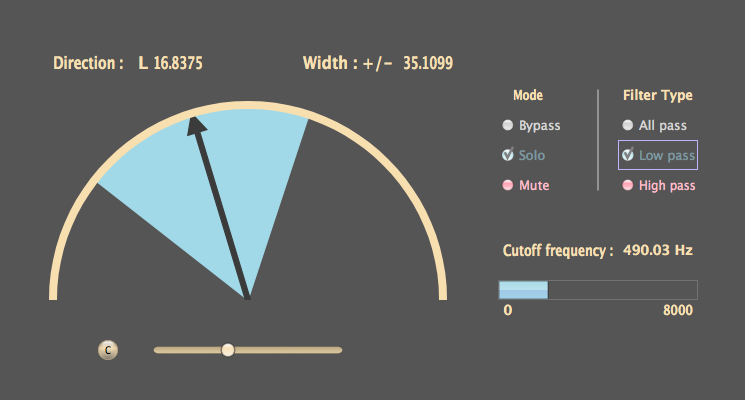
\includegraphics[width=.48\textwidth]{UI1}\quad
    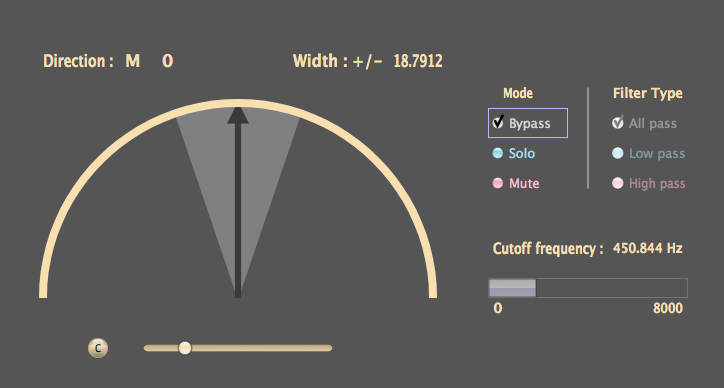
\includegraphics[width=.48\textwidth]{UI2}\\
    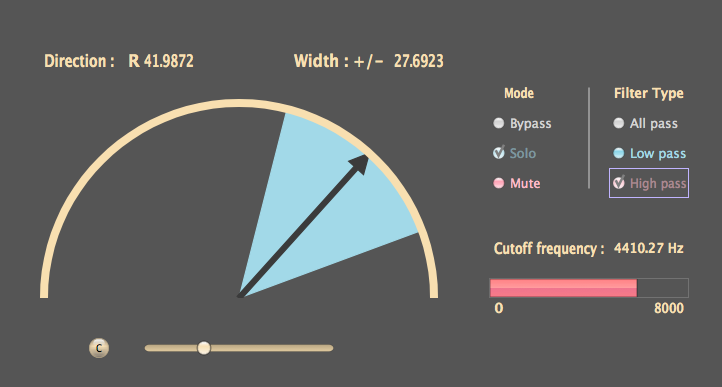
\includegraphics[width=.48\textwidth]{UI3}\quad
    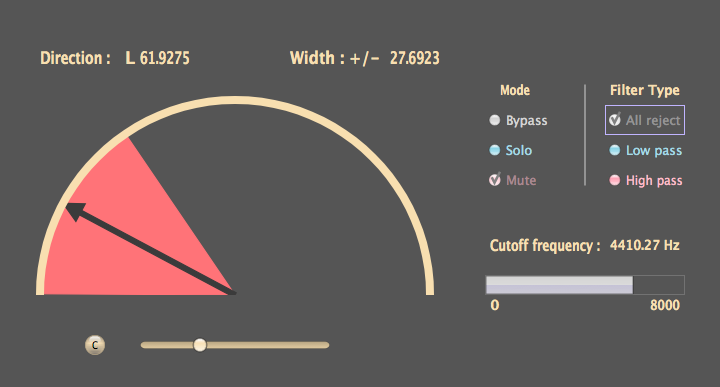
\includegraphics[width=.48\textwidth]{UI4}
    \caption{Plugin GUI for different modes}
    \label{fig:UI}
  \end{minipage}\\[1em]
\end{figure}
	

\section{Evaluation and Discussion}\label{sec:evaluation}

Although there are objective evaluations for source separation algorithms, they are abstract to some degree and not necessarily useful in this context of plugin development. We mainly look into the subjective sound quality and stability of the plugin for the evaluation of the project. 
    
The plugin has a 4096 block size and 3/4 overlapping rate, high enough for a reasonable sound quality after phase-vocoder processing. The signal is added Hann window and scale down by the factor of 2 when bypassing, or is added a Hanning resynthesized and added window again when conducting source separation, ensuring no distortion with bypassing few clips with resynthesized signal. There are typical phase-vocoder artifacts in the output, like the flickering grains of sound from isolate peaks in the spectrogram, or the bathroom-like artifacts. But by increasing the opening angle, the artifacts can be significantly reduced, bringing a much more natural sound.
     
The plugin has good stability and responds to user operations fairly quickly. There are few crashes in the final version of the plugin. When dragging the arrow and slides on the GUI, the components and parameters are reacting responsively. Thanks to the sensitive parameter change and the nature of ADRess itself, there are few clicks when changing the parameters.


\section{Conclusion and Future Work}\label{sec:conclusion}

This section will be edited later.

\section{Acknowledgement}\label{sec:acknowledgement}
Our thanks to Prof. Lerch for all the guidance and valuable advises.

\begin{thebibliography}{citations}

\bibitem {Barry:04}
Barry, Dan, Bob Lawlor, and Eugene Coyle.:
``Sound source separation: Azimuth discriminiation and resynthesis,''
{\it Proceedings of the 14th annual ACM international conference on Multimedia},
 ACM, 2004.


\end{thebibliography}


\end{document}
